% Sketch output, version 0.3 (build 2d, Wed Apr 20 23:38:45 2011)
% Output language: PGF/TikZ,LaTeX
\documentclass[letterpaper,12pt]{article}
\usepackage[x11names,rgb]{xcolor}
\usepackage{tikz}
\usetikzlibrary{snakes}
\usetikzlibrary{arrows}
\usetikzlibrary{shapes}
\usetikzlibrary{backgrounds}
\usepackage{amsmath}
\oddsidemargin 0in
\evensidemargin 0in
\topmargin 0in
\headheight 0in
\headsep 0in
\textheight 9in
\textwidth 6.5in
\begin{document}
\pagestyle{empty}
\vspace*{\fill}
\begin{center}
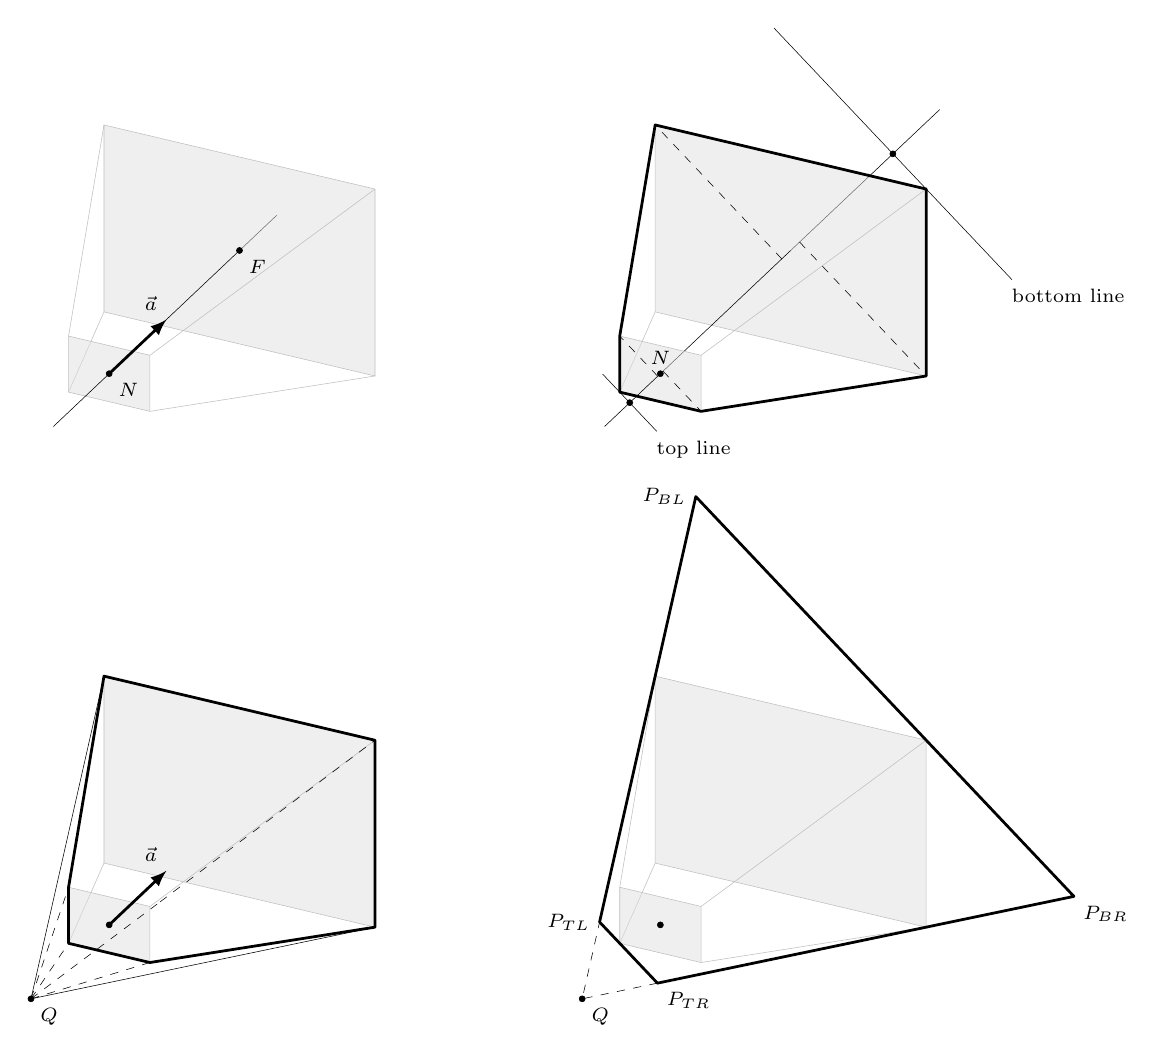
\begin{tikzpicture}[line join=round,line width=0.2pt,>=latex]
\draw(9.364,2.236)--(11.256,4.025);
\filldraw[color=lightgray,fill=lightgray!50,fill opacity=0.5](11.085,3.016)--(7.643,3.83)--(7.643,1.456)--(11.085,.642)--cycle;
\draw(2.364,2.236)--(2.837,2.683);
\filldraw[color=lightgray,fill=lightgray!50,fill opacity=0.5](4.085,3.016)--(.643,3.83)--(.643,1.456)--(4.085,.642)--cycle;
\draw[color=lightgray](.193,.437)--(.643,1.456);
\draw[color=lightgray](7.193,.437)--(7.643,1.456);
\filldraw[color=lightgray,fill=lightgray!50,fill opacity=0.5](4.085,-3.984)--(.643,-3.17)--(.643,-5.544)--(4.085,-6.358)--cycle;
\draw[color=lightgray](.193,-6.563)--(.643,-5.544);
\filldraw[color=lightgray,fill=lightgray!50,fill opacity=0.5](11.085,-3.984)--(7.643,-3.17)--(7.643,-5.544)--(11.085,-6.358)--cycle;
\draw[color=lightgray](7.193,-6.563)--(7.643,-5.544);
\draw[color=lightgray](7.193,1.149)--(7.643,3.83);
\draw[color=lightgray](.193,-5.851)--(.643,-3.17);
\draw(-.284,-7.268)--(.643,-3.17);
\draw[color=lightgray](7.193,-5.851)--(7.643,-3.17);
\draw[color=lightgray](.193,1.149)--(.643,3.83);
\draw(.709,.671)--(2.364,2.236);
\draw(7.709,.671)--(9.364,2.236);
\draw(-.284,-7.268)--(4.085,-6.358);
\draw[color=lightgray](1.226,-6.807)--(4.085,-6.358);
\draw[color=lightgray](8.226,.193)--(11.085,.642);
\draw[color=lightgray](1.226,.193)--(4.085,.642);
\draw[color=lightgray](8.226,-6.807)--(11.085,-6.358);
\draw[color=lightgray](8.226,.905)--(11.085,3.016);
\draw[color=lightgray](1.226,-6.095)--(4.085,-3.984);
\draw[dashed](1.355,-6.037)--(4.085,-3.984);
\draw[color=lightgray](8.226,-6.095)--(11.085,-3.984);
\draw[color=lightgray](1.226,.905)--(4.085,3.016);
\filldraw[color=lightgray,fill=lightgray!50,fill opacity=0.5](1.226,-6.095)--(.193,-5.851)--(.193,-6.563)--(1.226,-6.807)--cycle;
\filldraw[color=lightgray,fill=lightgray!50,fill opacity=0.5](8.226,.905)--(7.193,1.149)--(7.193,.437)--(8.226,.193)--cycle;
\filldraw[color=lightgray,fill=lightgray!50,fill opacity=0.5](1.226,.905)--(.193,1.149)--(.193,.437)--(1.226,.193)--cycle;
\draw[dashed](-.284,-7.268)--(.193,-6.563);
\filldraw[color=lightgray,fill=lightgray!50,fill opacity=0.5](8.226,-6.095)--(7.193,-5.851)--(7.193,-6.563)--(8.226,-6.807)--cycle;
\draw[dashed](-.284,-7.268)--(.193,-5.851);
\draw(7,0)--(7.709,.671);
\draw(0,0)--(.709,.671);
\draw[dashed](-.284,-7.268)--(1.226,-6.807);
\draw[dashed](-.284,-7.268)--(1.355,-6.037);
\filldraw(-.284,-7.268) circle (1.1pt);
\draw[solid](9.151,5.062)--(12.174,1.865);
\filldraw(10.662,3.463) circle (1.1pt);
\draw[dashed](9.477,2.343)--(11.085,.642);
\draw[dashed](9.251,2.129)--(7.643,3.83);
\draw[->,line width=1pt](.709,.671)--(1.436,1.358);
\draw[->,line width=1pt](.709,-6.329)--(1.436,-5.642);
\draw[dashed](7.743,.703)--(8.226,.193);
\draw[dashed](7.675,.639)--(7.193,1.149);
\draw[solid](6.976,.666)--(7.663,-.061);
\draw[dashed](7.672,-7.069)--(6.716,-7.268)--(6.937,-6.293);
\filldraw(7.32,.303) circle (1.1pt);
\filldraw[](.709,.671) circle (1.1pt);
\filldraw[](2.364,2.236) circle (1.1pt);

    \coordinate [label=290:\scriptsize$N$] (N) at (.709,.671);
    \coordinate [label=290:\scriptsize$F$] (F) at (2.364,2.236);
    \coordinate [label=175:\scriptsize$\vec{a}$] (a) at (1.436,1.358);
  \filldraw[](7.709,.671) circle (1.1pt);
\filldraw[fill=none,line width=1pt](7.643,3.83)--(7.193,1.149)--(7.193,.437)--(8.226,.193)--(11.085,.642)--(11.085,3.016)--cycle;

    \coordinate [label=90:\scriptsize$N$] (N) at (7.709,.671);
    \coordinate [label=-90:{\makebox[0pt][l]{\scriptsize top line}}] (top) at (7.663,-.061);
    \coordinate [label=-90:{\makebox[0pt][l]{\scriptsize bottom line}}] (bot) at (12.174,1.865);
  \filldraw[](.709,-6.329) circle (1.1pt);
\filldraw[fill=none,line width=1pt](.643,-3.17)--(.193,-5.851)--(.193,-6.563)--(1.226,-6.807)--(4.085,-6.358)--(4.085,-3.984)--cycle;

    \coordinate [label=-45:\scriptsize$Q$] (Q) at (-.284,-7.268);
    \coordinate [label=175:\scriptsize$\vec{a}$] (a) at (1.436,-5.642);
  \filldraw[](7.709,-6.329) circle (1.1pt);
\filldraw[](6.716,-7.268) circle (1.1pt);
\filldraw[fill=none,line width=1pt](6.937,-6.293)--(8.159,-.89)--(12.961,-5.967)--(7.672,-7.069)--cycle;

    \coordinate [label=-45:\scriptsize$Q$] (Q) at (6.716,-7.268);
    \coordinate [label=180:\scriptsize$P_{TL}$] (Ptl) at (6.937,-6.293);
    \coordinate [label=180:\scriptsize$P_{BL}$] (Pbl) at (8.159,-.89);
    \coordinate [label=-60:\scriptsize$P_{TR}$] (Ptr) at (7.672,-7.069);
    \coordinate [label=-60:\scriptsize$P_{BR}$] (Pbr) at (12.961,-5.967);
  \end{tikzpicture}
\end{center}
\vspace*{\fill}
\end{document}
% End sketch output
